\documentclass[/Users/ikedahajime/GitHub/reserch/master_report/thesis]{subfiles}
% このファイル内だけのコマンド
\begin{document}
\renewcommand{\prechaptername}{付録}
\renewcommand{\postchaptername}{}
\renewcommand{\thechapter}{\Alph{chapter}}
\setcounter{chapter}{0}

% \chapter{予備研究の結果}
\chapter{CABP系のスナップショット}\label{chap:cabp_snapshot}
\secref{sec:result_cabp}では高密度 CABP の閉じ込め系について論じた。%TODO:言い方
ここでは追加の本編で示していないスナップショットを示す。

\begin{figure}
    \centering
    \begin{tabular}{c}
        \begin{minipage}{0.45\hsize}
            \text{(a)}
            \includegraphics[width=\textwidth]{img/chiral/HAMLOD3_RAT40/volR20_Rc0.5.pdf}
        \end{minipage}
        \begin{minipage}{0.45\hsize}
            \text{(b)}
            \includegraphics[width=\textwidth]{img/chiral/HAMLOD3_RAT40/fai6R20_Rc0.5.pdf}
        \end{minipage}\\
        \begin{minipage}{0.45\hsize}
            \text{(c)}
            \includegraphics[width=\textwidth]{img/chiral/HAMLOD3_RAT40/volR20_Rc5.0.pdf}
        \end{minipage}
        \begin{minipage}{0.45\hsize}
            \text{(d)}
            \includegraphics[width=\textwidth]{img/chiral/HAMLOD3_RAT40/fai6R20_Rc5.0.pdf}
        \end{minipage}\\
        \begin{minipage}{0.45\hsize}
            \text{(e)}
            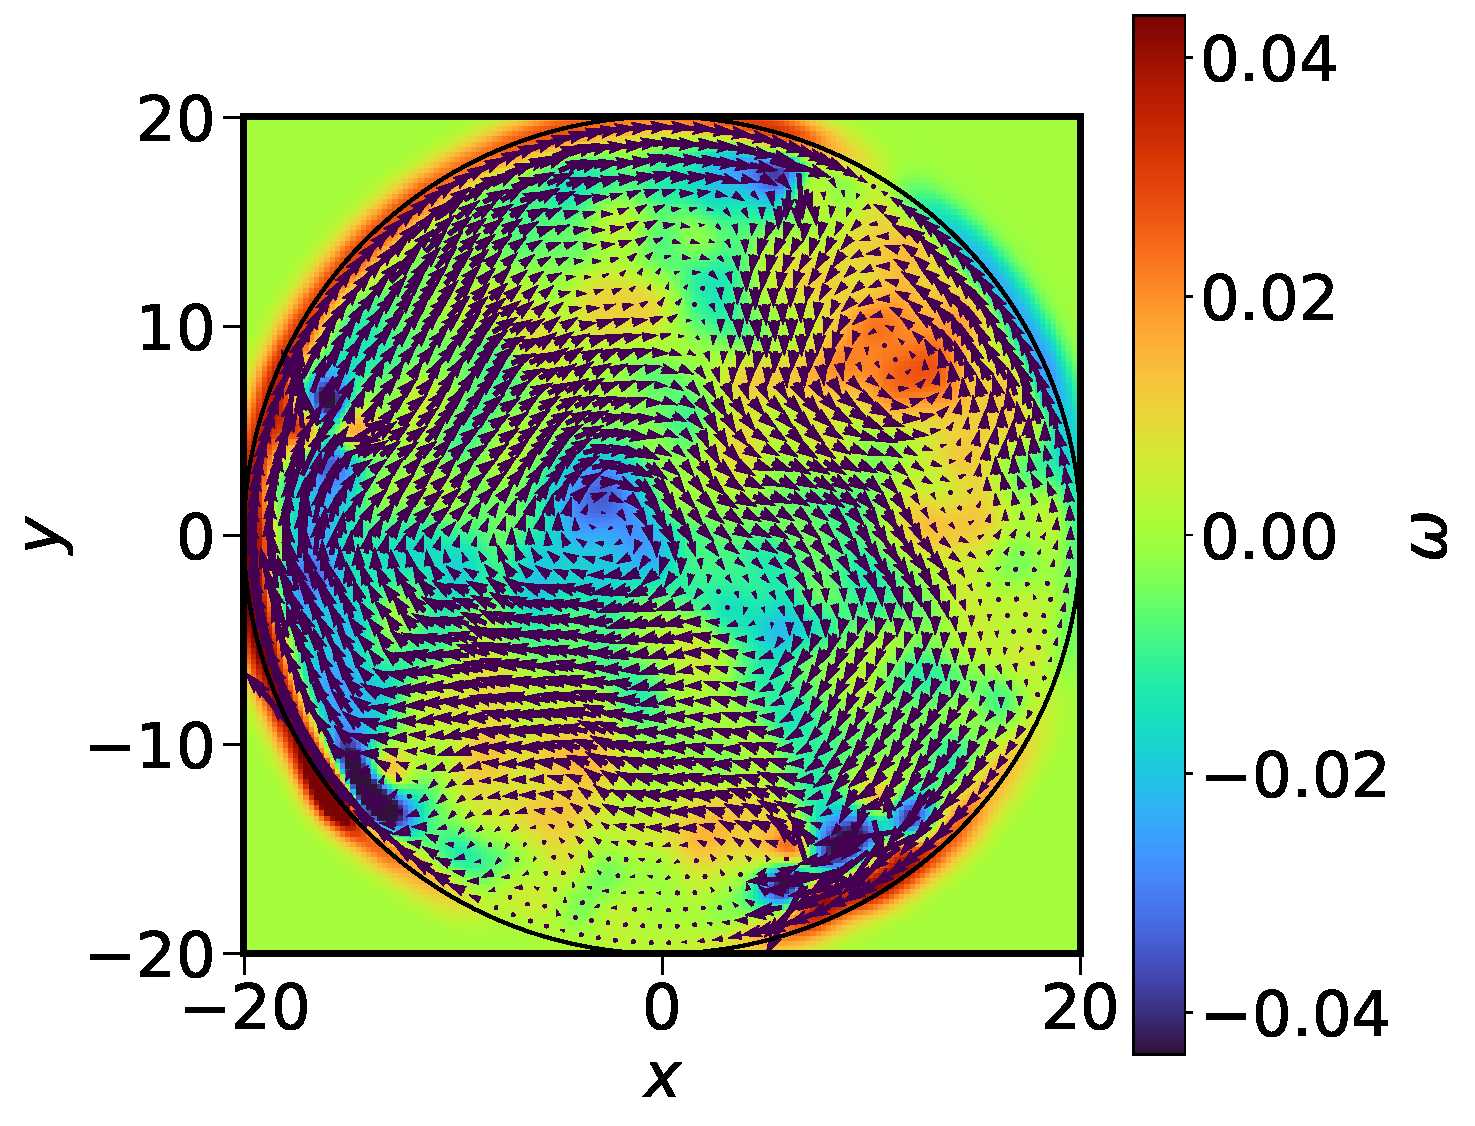
\includegraphics[width=\textwidth]{img/chiral/HAMLOD3_RAT40/volR20_Rc10.0.pdf}
        \end{minipage}
        \begin{minipage}{0.45\hsize}
            \text{(f)}
            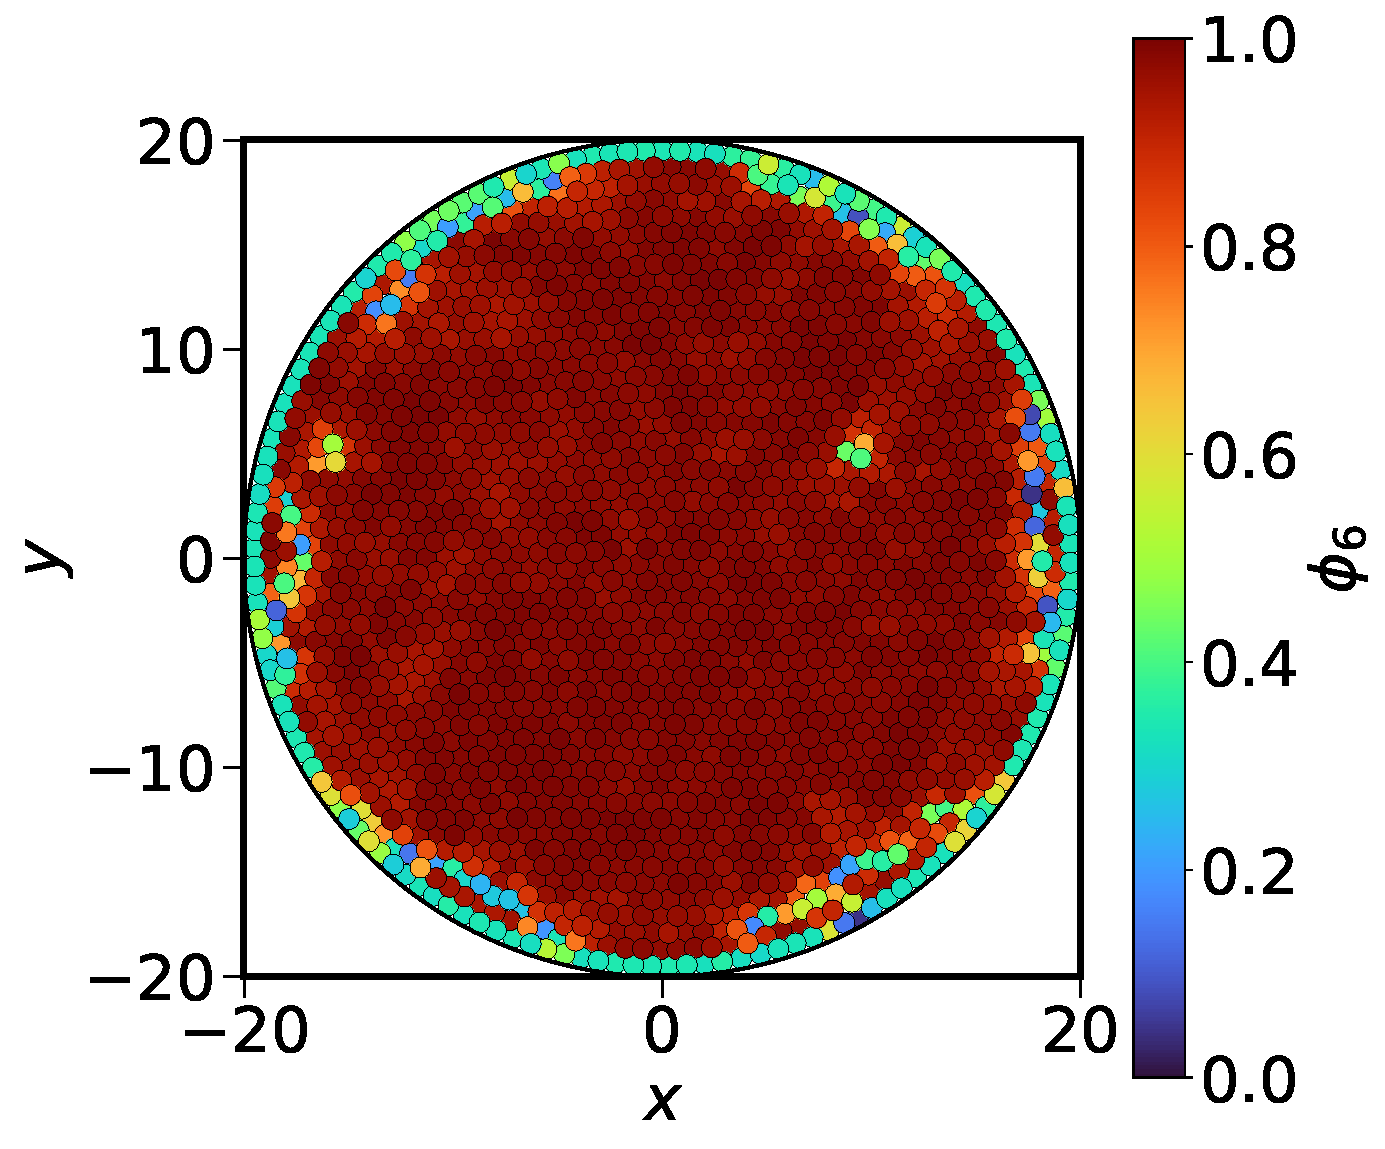
\includegraphics[width=\textwidth]{img/chiral/HAMLOD3_RAT40/fai6R20_Rc10.0.pdf}
        \end{minipage}
    \end{tabular}
    \caption[CABP_coor]
    {
        高密度CABPのスナップショット。設定は\figref{fig:CABP_coor}と同様である。
        (a)、(b) では$R_\Omega=0.5$、(c)、(d) では、$R_\Omega=5$、
        (e)、(f) では$R_\Omega=10$を用いた。
    }
    \label{fig:CABP_coor_app1}
\end{figure}

\begin{figure}
    \centering
    \begin{tabular}{c}
        \begin{minipage}{0.45\hsize}
            \text{(a)}
            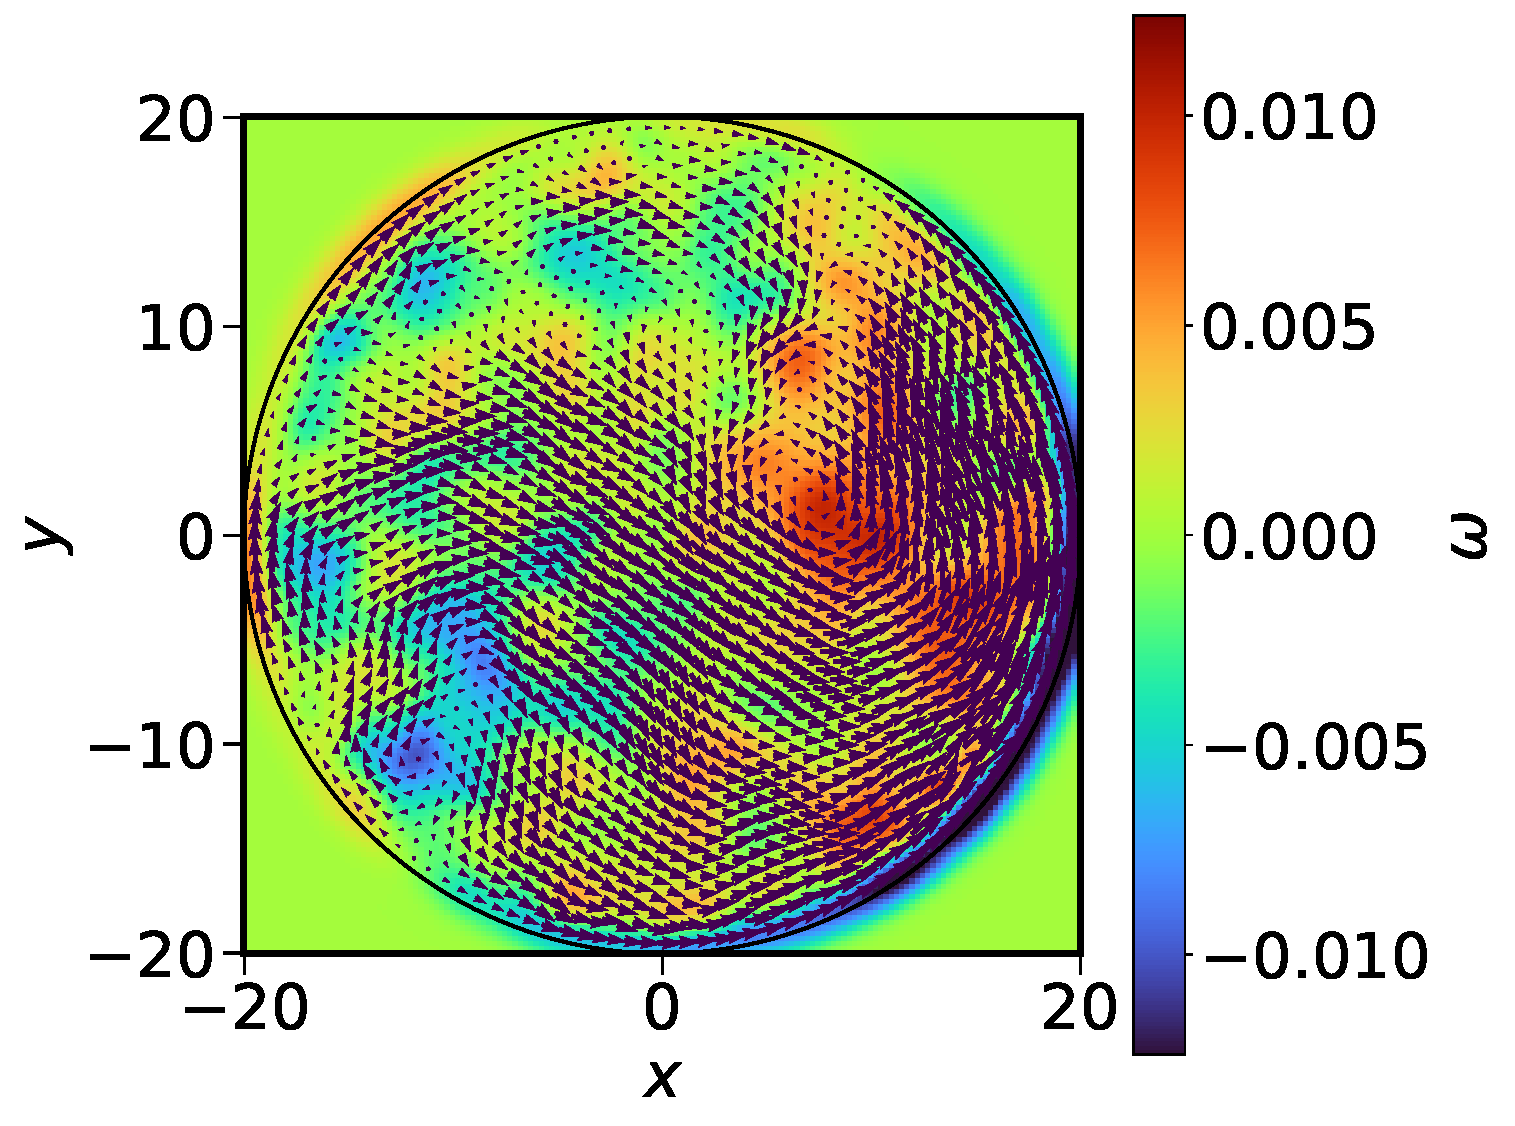
\includegraphics[width=\textwidth]{img/chiral/HAMLOD3_RAT40/volR20_Rc26.667.pdf}
        \end{minipage}
        \begin{minipage}{0.45\hsize}
            \text{(b)}
            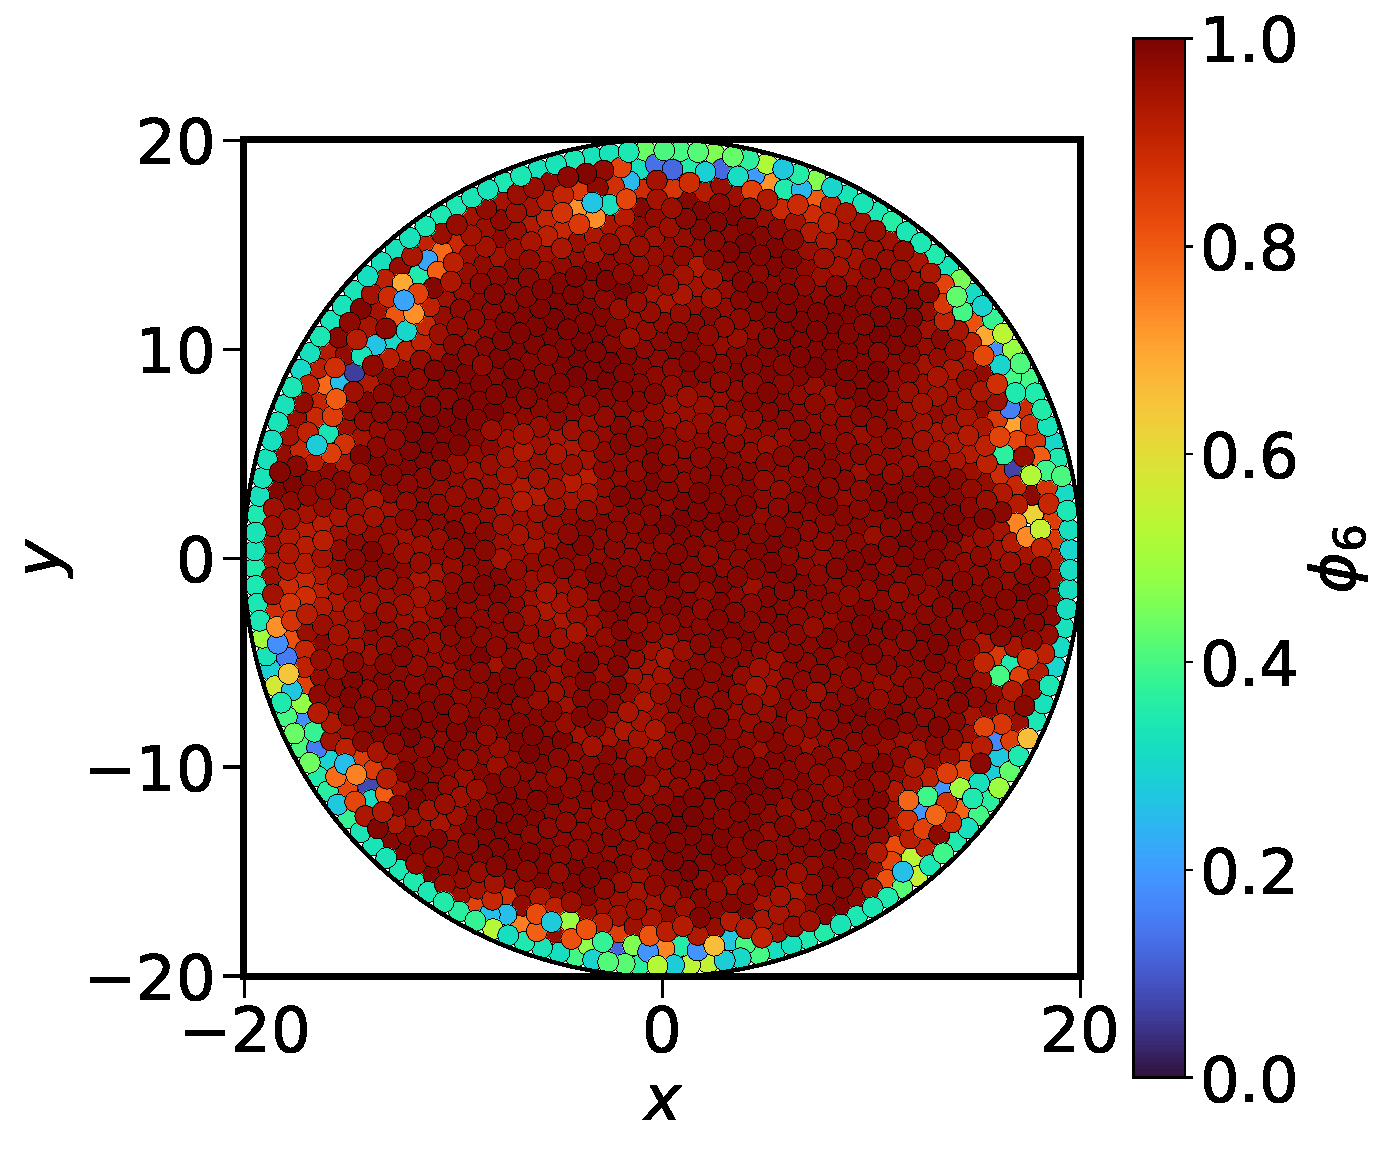
\includegraphics[width=\textwidth]{img/chiral/HAMLOD3_RAT40/fai6R20_Rc26.667.pdf}
        \end{minipage}\\
        \begin{minipage}{0.45\hsize}
            \text{(c)}
            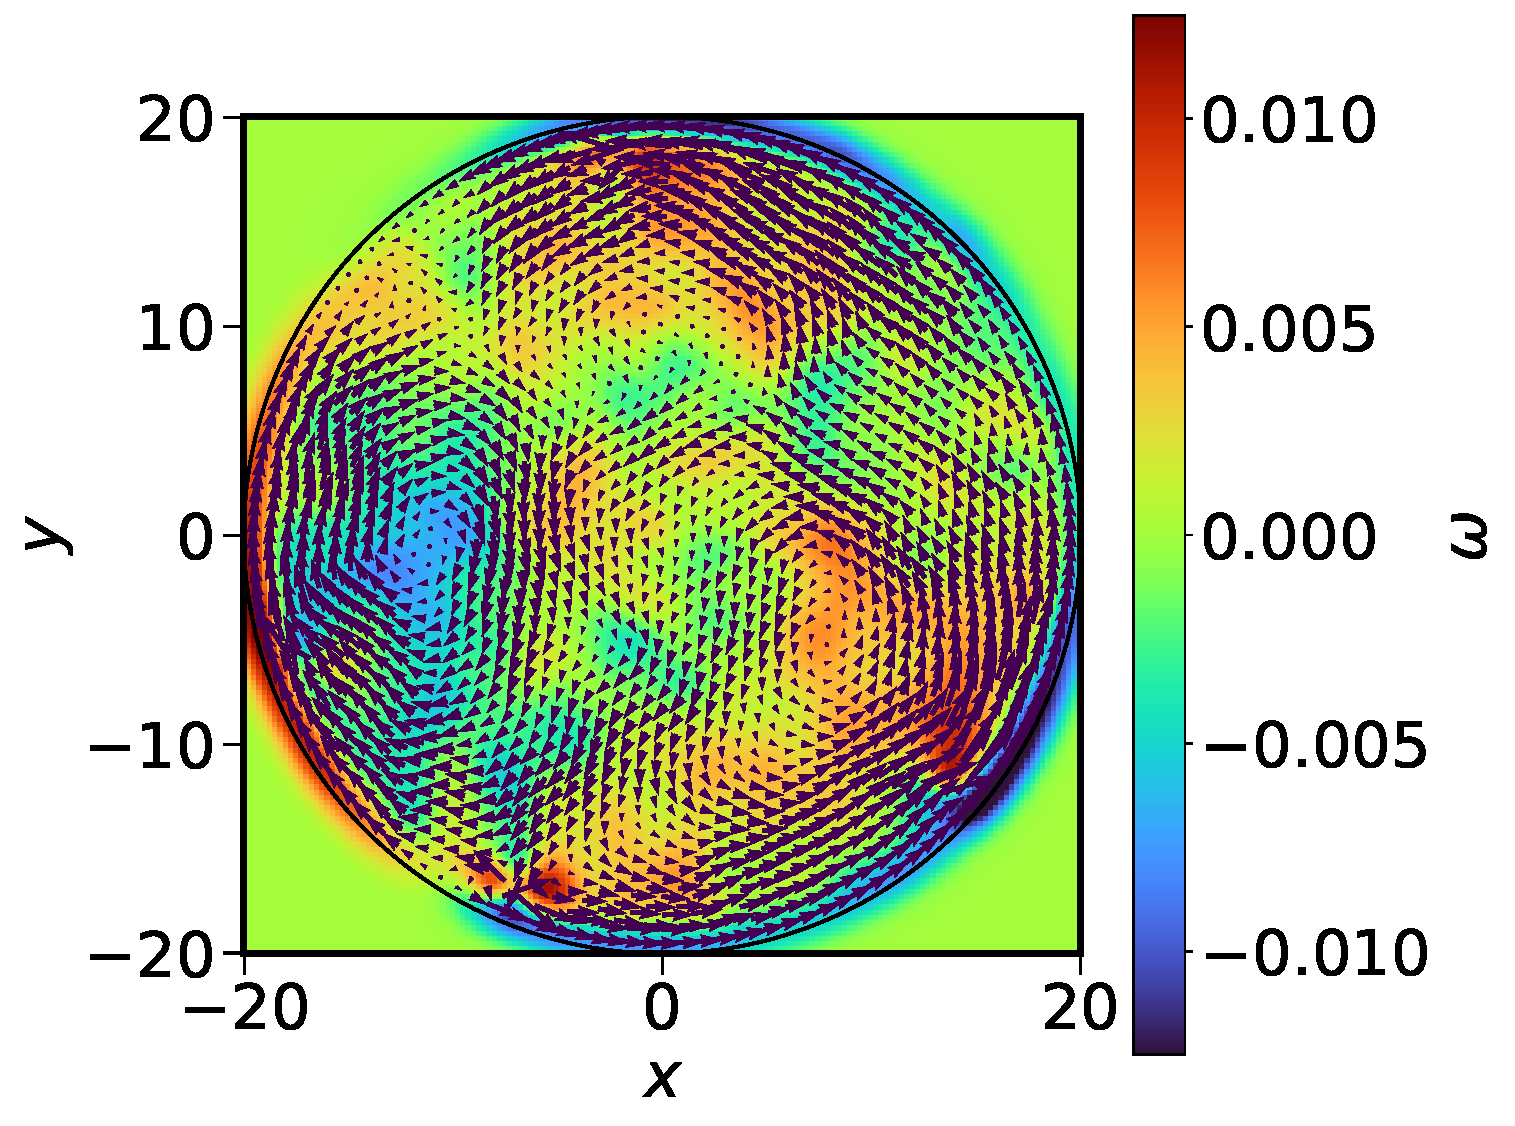
\includegraphics[width=\textwidth]{img/chiral/HAMLOD3_RAT40/volR20_Rc33.333.pdf}
        \end{minipage}
        \begin{minipage}{0.45\hsize}
            \text{(d)}
            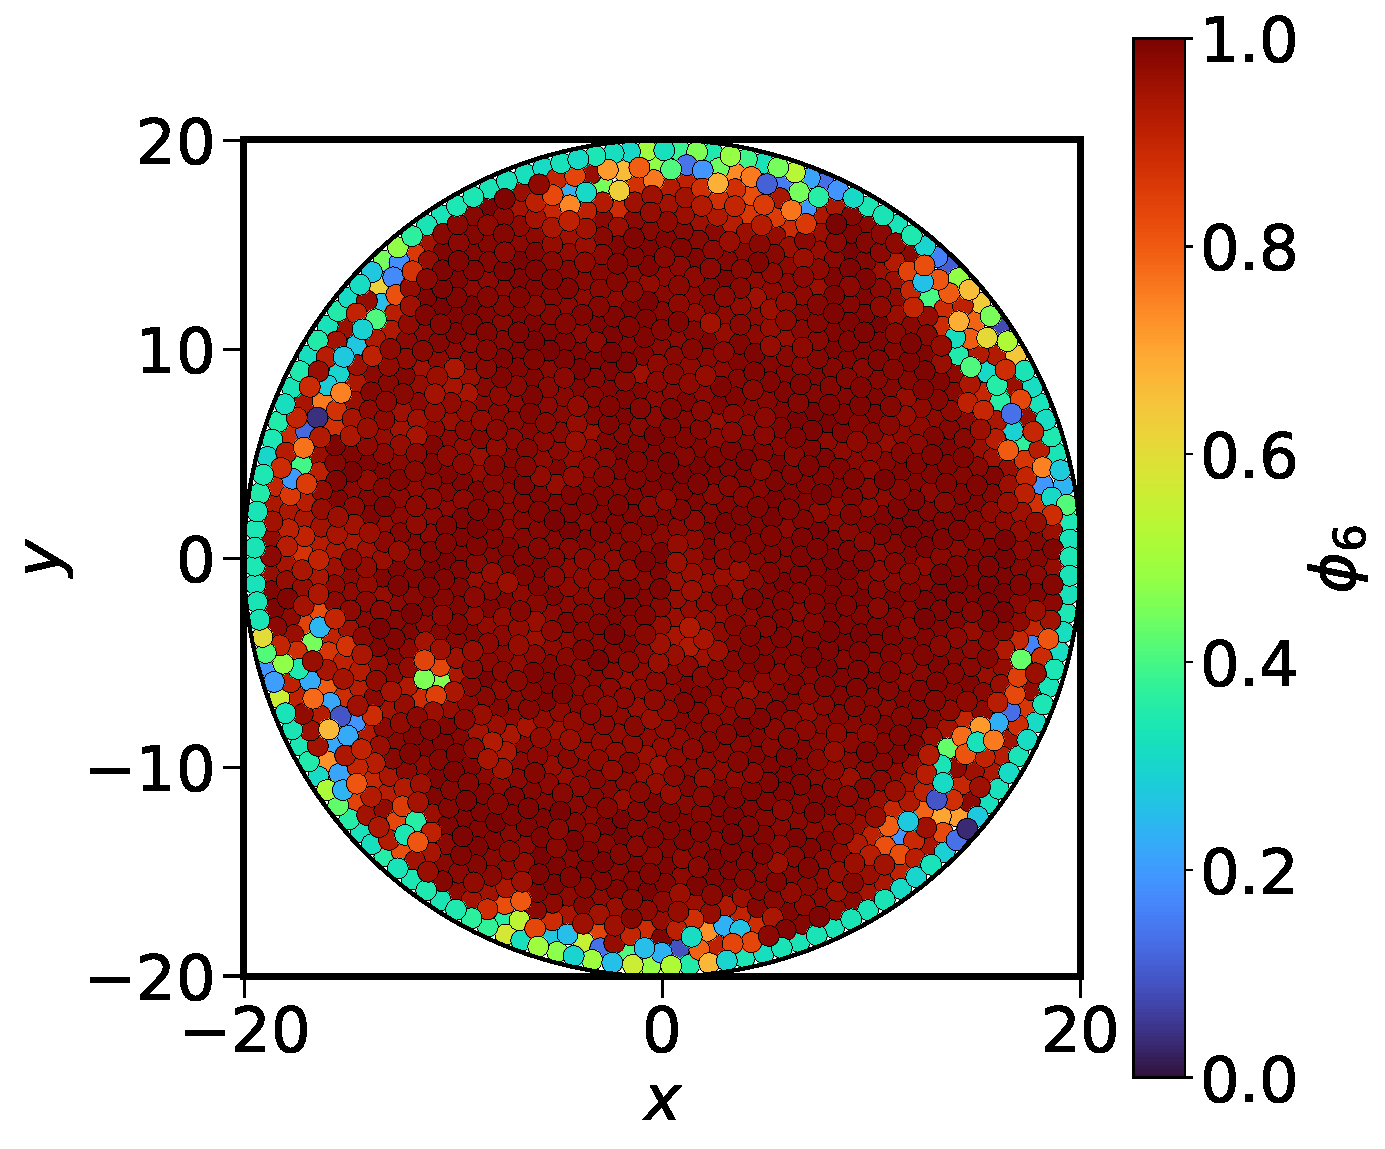
\includegraphics[width=\textwidth]{img/chiral/HAMLOD3_RAT40/fai6R20_Rc33.333.pdf}
        \end{minipage}\\
        \begin{minipage}{0.45\hsize}
            \text{(e)}
            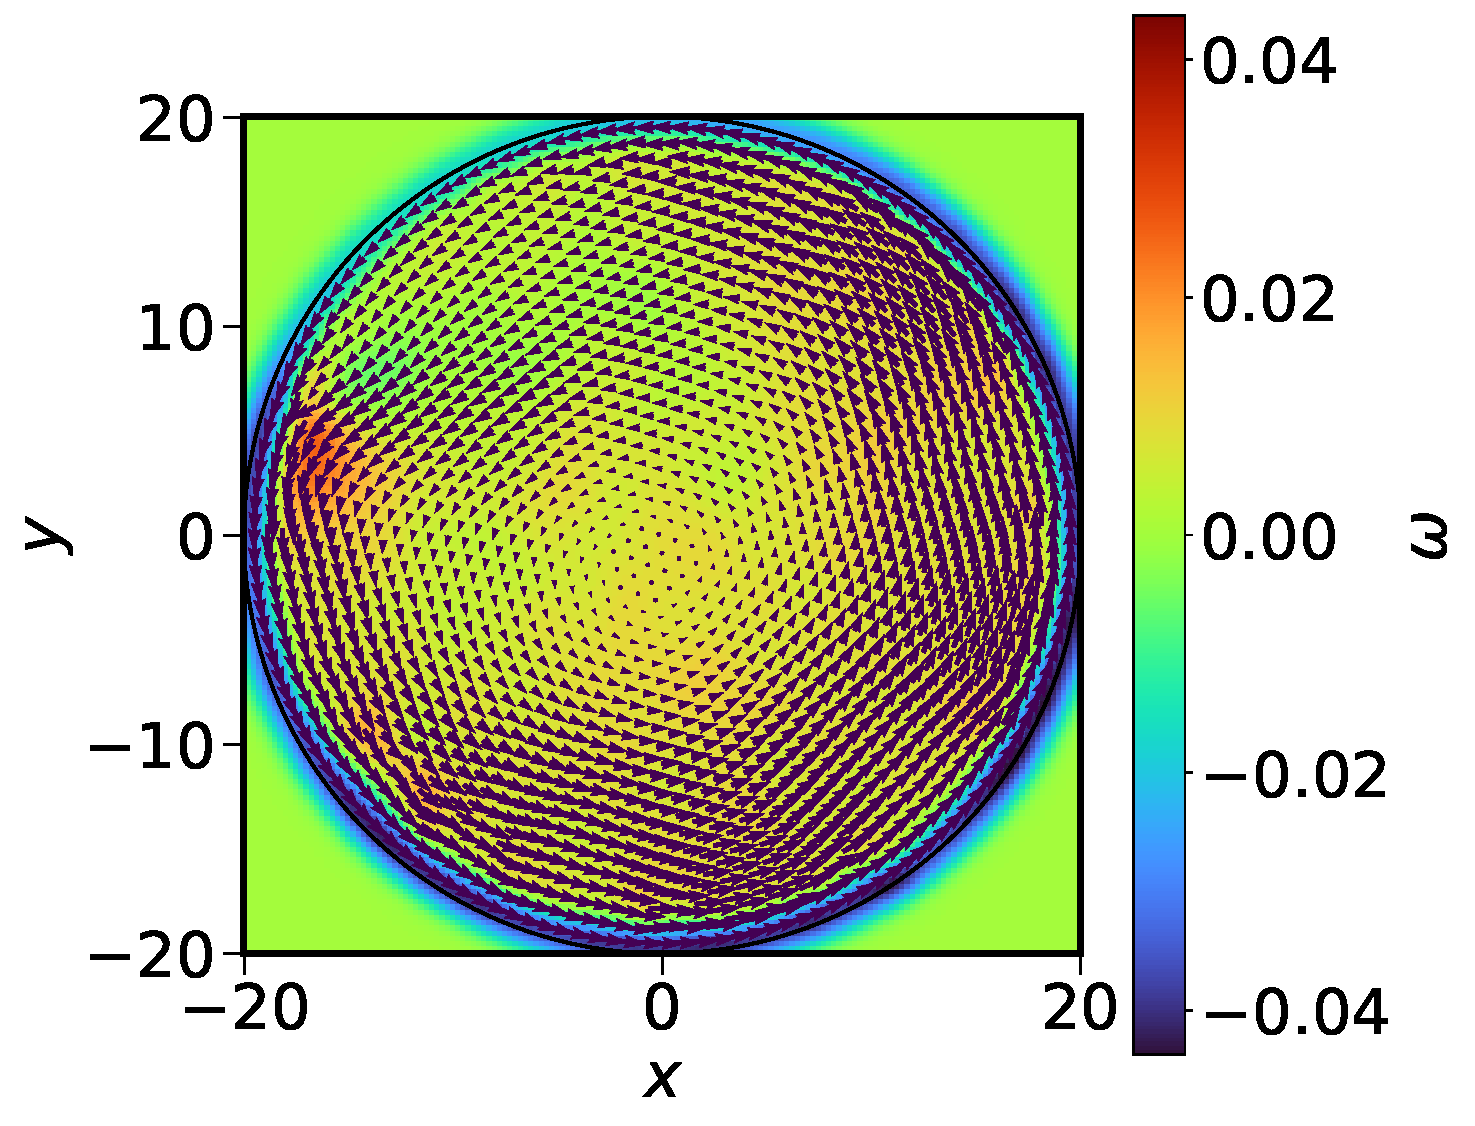
\includegraphics[width=\textwidth]{img/chiral/HAMLOD3_RAT40/volR20_Rc40.0.pdf}
        \end{minipage}
        \begin{minipage}{0.45\hsize}
            \text{(f)}
            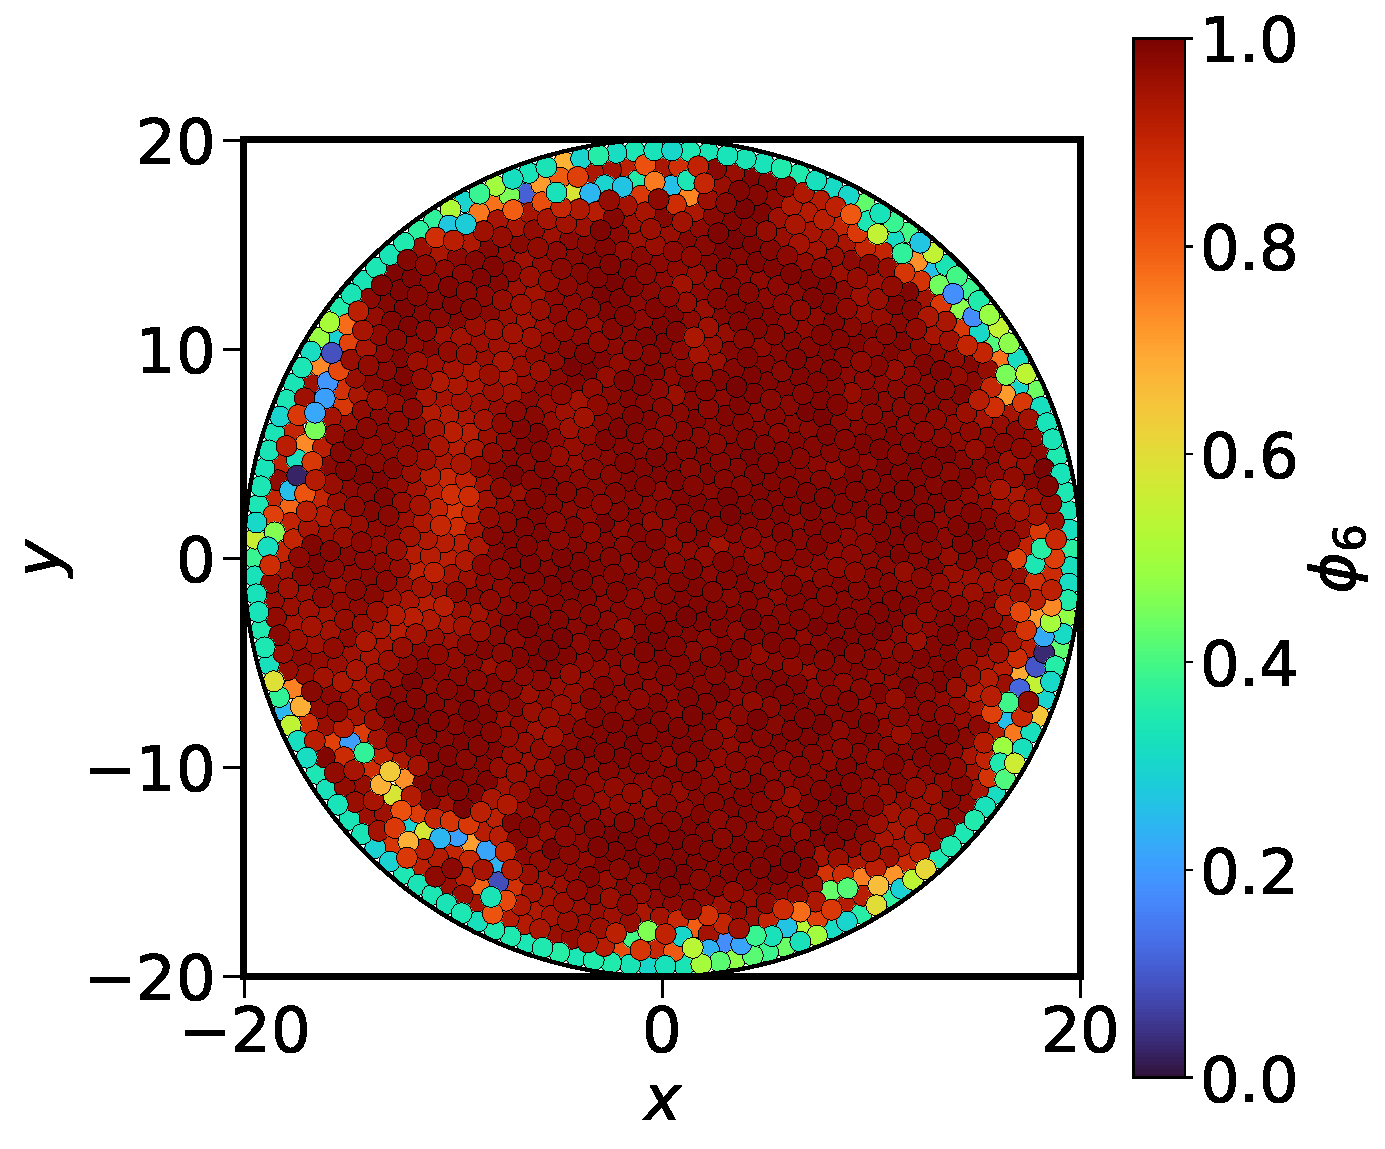
\includegraphics[width=\textwidth]{img/chiral/HAMLOD3_RAT40/fai6R20_Rc40.0.pdf}
        \end{minipage}
    \end{tabular}
    \caption[CABP_coor]
    {
        高密度CABPのスナップショット。設定は\figref{fig:CABP_coor}と同様である。
        (a)、(b) では$R_\Omega=26.7$、(c)、(d) では、$R_\Omega=33.3$、
        (e)、(f) では$R_\Omega=40$を用いた。
    }
    \label{fig:CABP_coor_app2}
\end{figure}
\begin{figure}
    \centering
    \begin{tabular}{c}
        \begin{minipage}{0.45\hsize}
            \text{(a)}
            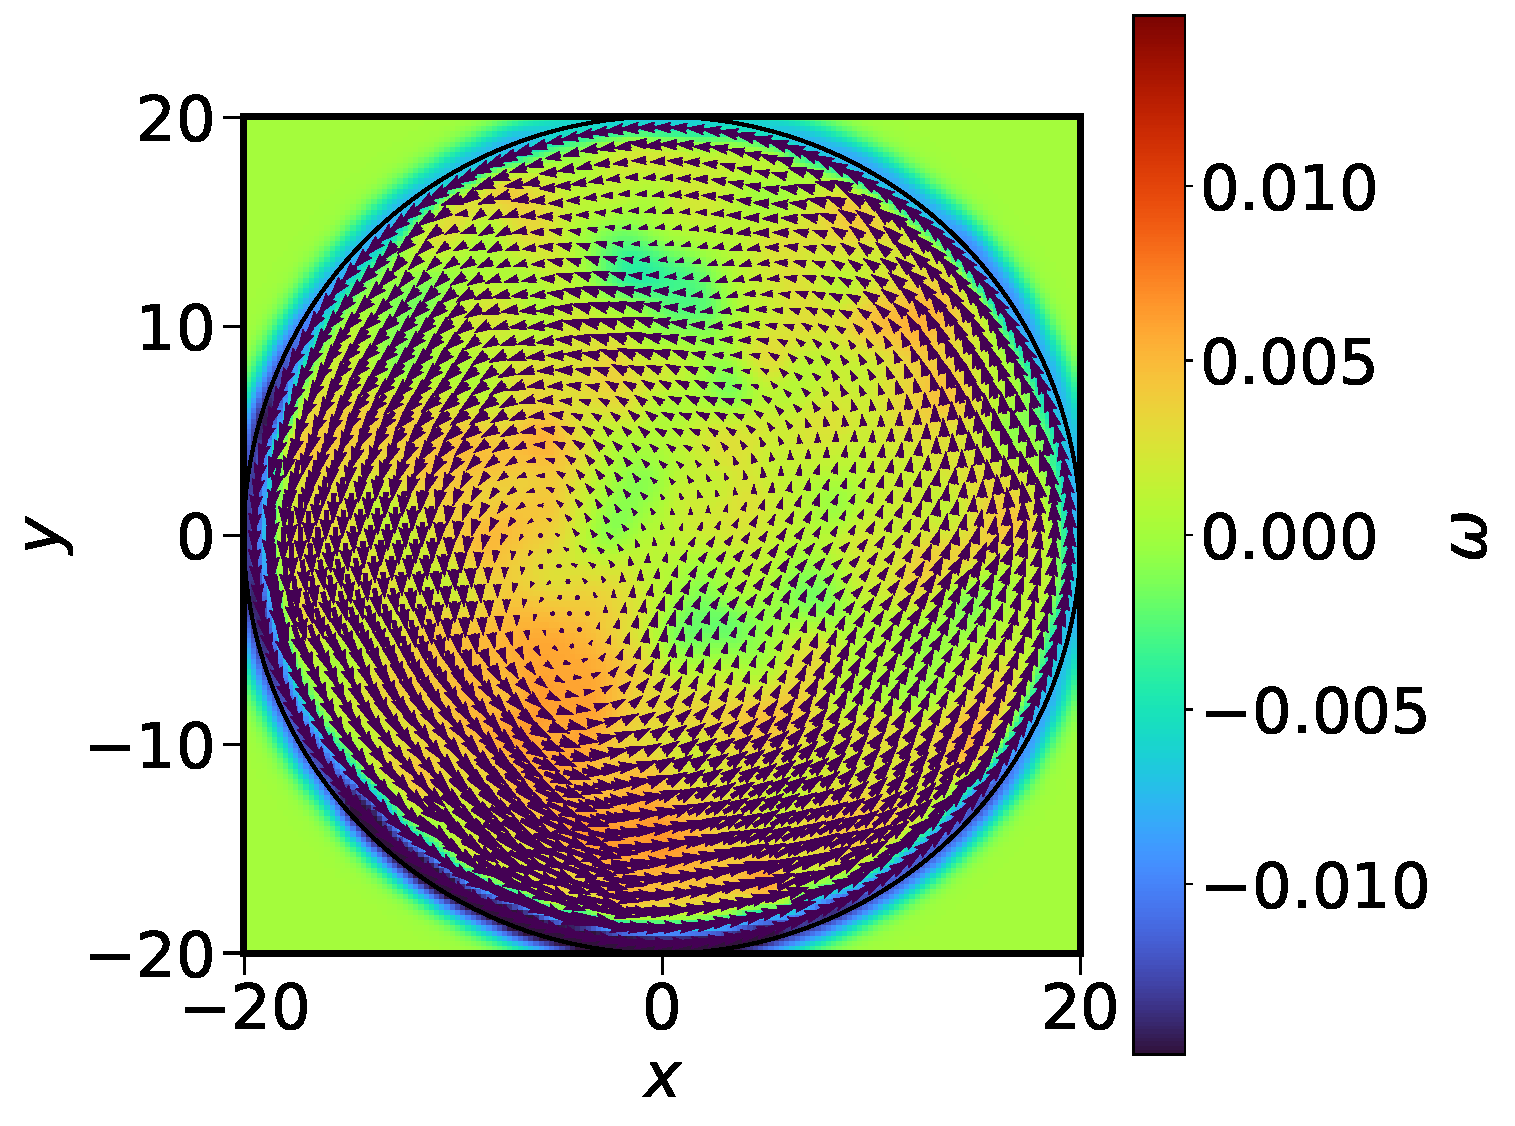
\includegraphics[width=\textwidth]{img/chiral/HAMLOD3_RAT40/volR20_Rc50.0.pdf}
        \end{minipage}
        \begin{minipage}{0.45\hsize}
            \text{(b)}
            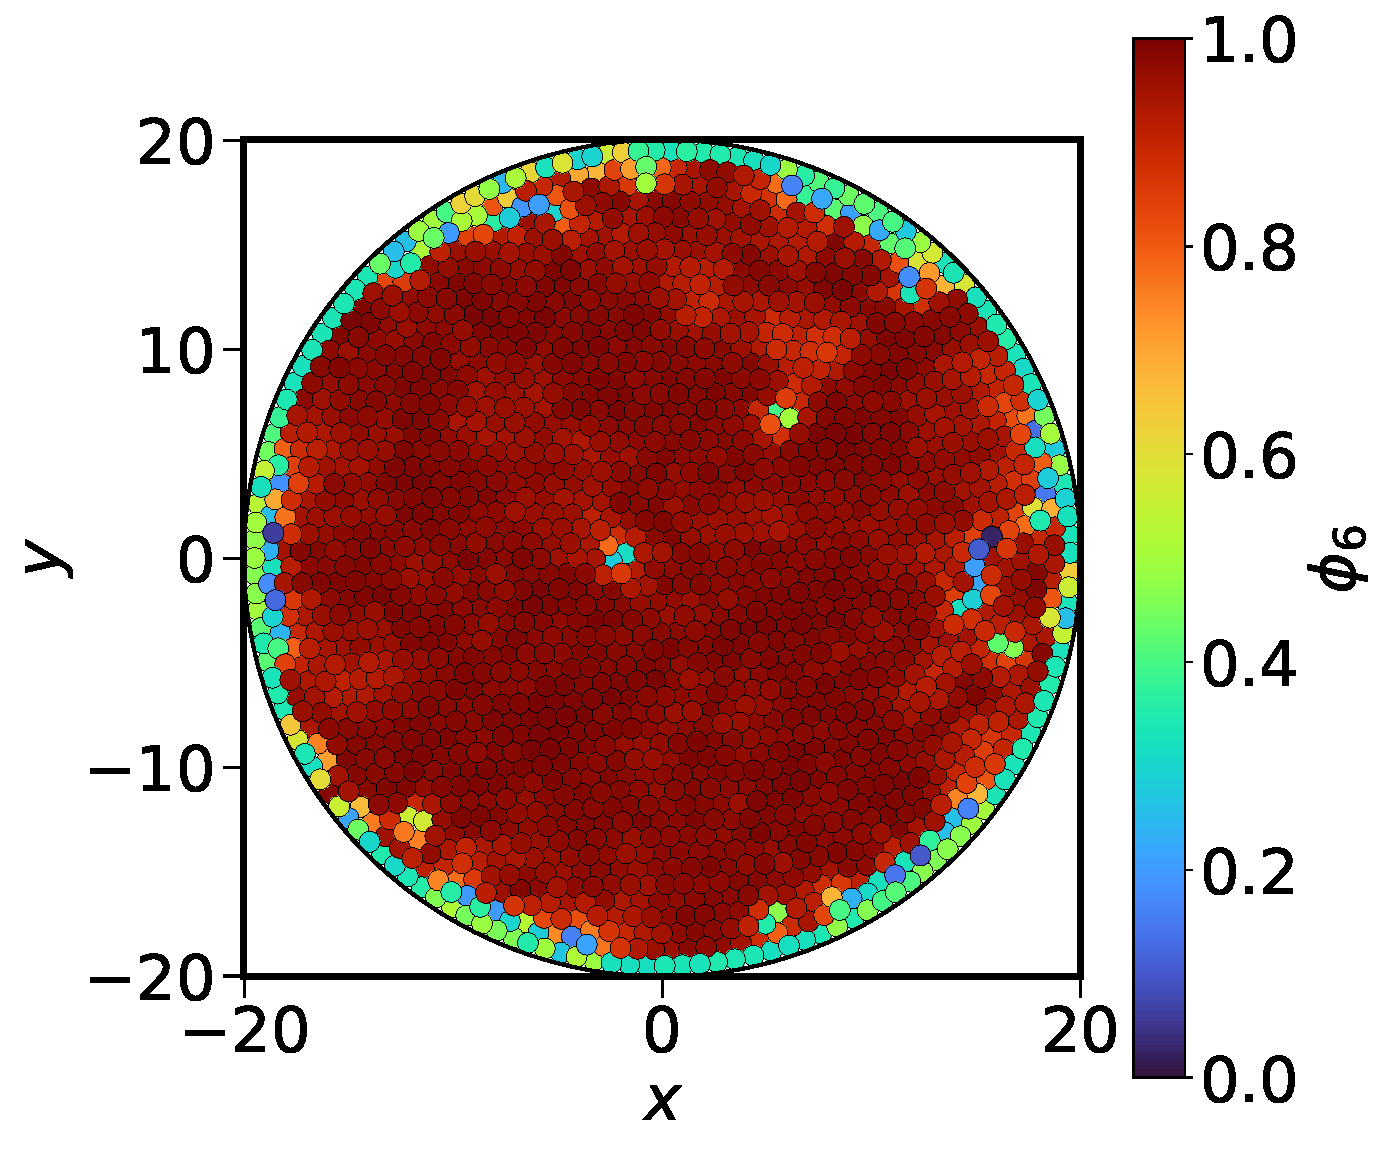
\includegraphics[width=\textwidth]{img/chiral/HAMLOD3_RAT40/fai6R20_Rc50.0.pdf}
        \end{minipage}\\
        \begin{minipage}{0.45\hsize}
            \text{(c)}
            \includegraphics[width=\textwidth]{img/chiral/HAMLOD3_RAT40/volR20_Rc200.0.pdf}
        \end{minipage}
        \begin{minipage}{0.45\hsize}
            \text{(d)}
            \includegraphics[width=\textwidth]{img/chiral/HAMLOD3_RAT40/fai6R20_Rc200.0.pdf}
        \end{minipage}\\
        \begin{minipage}{0.45\hsize}
            \text{(e)}
            \includegraphics[width=\textwidth]{img/chiral/HAMLOD3_RAT40/volR20_Rc300.0.pdf}
        \end{minipage}
        \begin{minipage}{0.45\hsize}
            \text{(f)}
            \includegraphics[width=\textwidth]{img/chiral/HAMLOD3_RAT40/fai6R20_Rc300.0.pdf}
        \end{minipage}
    \end{tabular}
    \caption[CABP_coor]
    {
        高密度CABPのスナップショット。設定は\figref{fig:CABP_coor}と同様である。
        (a)、(b) では$R_\Omega=50$、(c)、(d) では、$R_\Omega=200$、
        (e)、(f) では$R_\Omega=300$を用いた。
    }
    \label{fig:CABP_coor_app3}
\end{figure}

\end{document}
